%%%%%%%%%%%%%%%%%%%%%%%%%%%%%%%%%%%%%%%%%
% fphw Assignment
% LaTeX Template
% Version 1.0 (27/04/2019)
%
% This template originates from:
% https://www.LaTeXTemplates.com
%
% Authors:
% Class by Felipe Portales-Oliva (f.portales.oliva@gmail.com) with template 
% content and modifications by Vel (vel@LaTeXTemplates.com)
%
% Template (this file) License:
% CC BY-NC-SA 3.0 (http://creativecommons.org/licenses/by-nc-sa/3.0/)
%
%%%%%%%%%%%%%%%%%%%%%%%%%%%%%%%%%%%%%%%%%

%----------------------------------------------------------------------------------------
%	PACKAGES AND OTHER DOCUMENT CONFIGURATIONS
%----------------------------------------------------------------------------------------

\documentclass[
	french,
	11pt, % Default font size, values between 10pt-12pt are allowed
	%letterpaper, % Uncomment for US letter paper size
	%spanish, % Uncomment for Spanish
]{fphw}

% Template-specific packages
\usepackage{babel}
\usepackage[utf8]{inputenc} % Required for inputting international characters
\usepackage[T1]{fontenc} % Output font encoding for international characters
\usepackage{mathpazo} % Use the Palatino font
% \usepackage{iwona} % Use the Iwona font
% \usepackage[T1]{fontenc}
% \usepackage{iwona}    %% Roman text font 
% \usepackage{mathdots}
% \usepackage{eulervm}

\usepackage{amsmath}
\usepackage{mathtools}
\usepackage{cases}	% Required to use nmbered tags in cases

\usepackage{graphicx} % Required for including images
\usepackage{caption}  %% To manage long captions in images
\usepackage{subcaption}
\usepackage{float}
\graphicspath{ {./img/} }
\captionsetup{justification=centering}

\usepackage{booktabs} % Required for better horizontal rules in tables

\usepackage{listings} % Required for insertion of code

\usepackage{array} % Required for spacing in tabular environment

\usepackage{enumerate} % To modify the enumerate environment

\usepackage{amssymb}
\usepackage{enumitem}	%% % To modify the itemize bullet character

\usepackage[linkcolor=blue,colorlinks=true]{hyperref}
\usepackage{cleveref}  %% To make links clickable

\newcommand{\hquad}{\hspace{0.5em}} %% Bew command for half quad
\usepackage{indentfirst}	%% Indent the first paragraph
\newcommand{\bi}{\text{Bi}} 
\newcommand{\bvec}[1]{\bm{#1}}    %% For vector notation
\newcommand{\myvec}[2]{\begin{pmatrix} #1  \\ #2 \end{pmatrix}}   %% vecteur 2d
\newcommand{\mymat}[4]{\begin{pmatrix} #1 & #2 \\ #3 & #4 \end{pmatrix}}  %% Matrice 2*2


%----------------------------------------------------------------------------------------
%	ASSIGNMENT INFORMATION
%----------------------------------------------------------------------------------------

\title{T.P \#1} % Assignment title

\author{Roussel Desmond Nzoyem} % Student name

\date{\today} % Due date

\institute{Université de Strasbourg \\ UFR de Mathématiques et Informatique} % Institute or school name

\class{contrôle optimal} % Course or class name

\professor{Pr. Yannick Privat} % Professor or teacher in charge of the assignment

%----------------------------------------------------------------------------------------

\begin{document}

\maketitle % Output the assignment title, created automatically using the information in the custom commands above

%----------------------------------------------------------------------------------------
%	ASSIGNMENT CONTENT - SECTION 1
%----------------------------------------------------------------------------------------

\section*{Exercice 1 - Préliminaires}

\subsection*{Question}

\begin{problem}

Résolution théorique, puis numérique du problème
\begin{align*}
\begin{cases}
\inf_{K} J \\
\text{avec} \quad J: \mathbb{R}\times\mathbb{R} \to \mathbb{R} \\
(x_1, x_2) \mapsto x_1^2 + x_2^2 - 14x_1 - 6x_2 - 7 \\ 
% \end{align*}
% \begin{align*}
\text{et} \\
K = \{(x_1, x_2) \in \mathbb{R}^2 \, | \, g_1(x_1,x_2) \leq 0 \, \text{   et   } g_2(x_1,x_2) \leq 0 \} \\
\text{où  } \quad g_1(x_1,x_2) = x_1 + x_2 -2 \quad \text{et} \quad g_2(x_1,x_2) = x_1 + 2x_2 -3
\end{cases}
\end{align*}

\end{problem}

\subsection*{Réponse}

On écrit, pour $x=(x_1,x_2) \in \mathbb{R}$
\begin{align*}
J(x_1, x_2) &= x_1^2 + x_2^2 - 14x_1 - 6x_2 - 7 \\
&= \frac{1}{2} \langle Ax,x \rangle - \langle b,x \rangle - c
\end{align*}
avec 
\begin{align*}
	A &= \mymat{2}{0}{0}{2} = 2I_2 \in S_2^{++} \\
	b &= \left(14,6\right) ^\bot \\
	c &= 7
\end{align*}
On remarque
\begin{itemize}
	\item J est $C^0$ car polynomiale
	\item J est coercive car $A \in S_2^{++}$
	\item K est fermé
\end{itemize}

L'existence d'un minimiseur est donc garantie; et les contraintes sont qualifiées. En effet, la famille $\left( \nabla g_1(x), \nabla g_2(x) \right) = \left( \myvec{1}{2}, \myvec{1}{2} \right)$ est libre dans $K$. Appliquons le théorème de Kuhn-Tucker.
$\exists \, ( \lambda_1, \lambda_2 ) \in \mathbb{R}^2_+$ tel que
\begin{align*}
	\begin{cases}
		\nabla J(x_1, x_2) + \lambda_1 \nabla g_1(x_1,x_2) + \lambda_2 \nabla g_2(x_1,x_2) =0 \\
		\lambda_1 g_1(x_1,x_2)=0 \\
		\lambda_2 g_2(x_1,x_2)=0 \\
		g_1(x_1,x_2) \leq 0 \\
		g_2(x_1,x_2) \leq 0
	\end{cases}
\end{align*} 
Soit encore
\begin{numcases}{}
	\myvec{2x_1}{2x_2} + \lambda_1 \myvec{1}{1} + \lambda_2 \myvec{1}{2} =0 \\
	\lambda_1 (x_1+x_2-2)=0 \\
	\lambda_2 (x_1+2x_2-3)=0 \\
	g_1(x_1,x_2) \leq 0 \\
	g_2(x_1,x_2) \leq 0
\end{numcases}

\begin{itemize}
	\item[$\blacksquare$] Si $\lambda_1 \neq 0$, alors $(3) \Rightarrow x_1+x_2-2=0 \Rightarrow x_1 = x_2+2 $ 
	$$(4) \Rightarrow \lambda_2(x_2-1)=0$$ 
	\begin{itemize} 
		\item Si $\lambda_2 \neq 0$ alors $\mathbf{(x_1,x_2)=(1,1)}$ 
		\item Si $\lambda_2 = 0$ alors $(1) \Rightarrow$ $\mathbf{(x_1,x_2)=(3,-1)}$
	\end{itemize}
	\item[$\blacksquare$] Si $\lambda_1 = 0$
	\begin{itemize}
		\item Si $\lambda_2 \neq 0$, alors $(3) \Rightarrow x_1 = -2x_2+3$, et $(1) \Rightarrow$ $(x_1,x_2) =(5,-1)$. Mais d'après (4), $g_1(5,-1)=2 \nleq 0$
		\item Si $\lambda_2 = 0$, $(1) \Rightarrow (x_1,x_2)=(7,3)$. Mais $g_1(7,3)=8 \nleq 0$
	\end{itemize} 
\end{itemize}

On obtient au final deux candidats: $(x_1,x_2)=(1,1)$ et $(x_1,x_2)=(3,-1)$. $J(1,1)=-25 > -33=J(3,-1)$. On conclut que le minimiseur de $J$ est le vecteur $x=(3,-1)^\perp $, ce qui est confirmé par le code Gekko: 
\begin{align*}
	x:& [2.9999999999] \\
	y:& [-1.0000000066]
\end{align*}



\clearpage


\section*{Exercice 2 - Contrôle d'un tram}

\begin{problem}
	Le problème du contrôle du tram est modélisé par:
	\begin{align}
		\begin{cases}
			x^\prime(t) = y(t) \\
			y^\prime(t) = u(t) \\
			x(0)=0,\, y(0)=0
		\end{cases}
		\label{eq:exo3}
	\end{align}	

\end{problem}


\subsection*{1ère version}
On voudrait avoir $x(T)=0$, $y(T)=-1$, sous la contrainte $\vert u(t) \vert \leq 1$ p.p. $t \in ]0,T[$.
 
Le résultat obtenu (\cref{fig:Exo21}) indique un temps minimal égal à $T=2.3979143983$, cela à travers un contrôle bang-bang.
\begin{figure}[H]
    \centering
    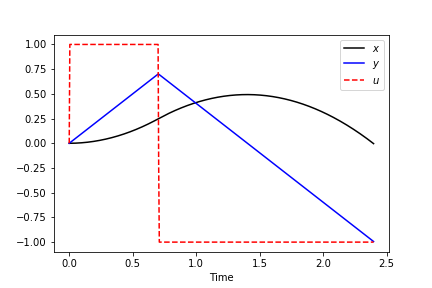
\includegraphics[width=0.5\textwidth]{Exo2Ver1.png}
	\caption{Résultat obtenu pour le problème temps optimal pour le contrôle du tram}
	\label{fig:Exo21}
\end{figure}
Vu que le contrôle représente l'accélération (puissance du tram), l'objectif pour le tram est de retourner à sa position de départ avec une vitesse de $y(T)=-1$. La stratégie consiste à accélérer au départ ($u=1$), ensuite de décélérer ($u=-1$) afin d'arriver en $x(T)=0$ avec une vitesse réduites.


\subsection*{2ème version}
On pose $z(t)= \frac{1}{2} ( x^\prime(t)^2 + x(t)^2) $, le problème revient à résoudre $\inf_{u\in \cal U} (\xi T + (1-\xi)z(T))$ ou $\xi \in [0,1]$ et les contraintes
\begin{align*}
x^\prime (t)&=y(t) \\
y^\prime (t)&=u(t) \\
z^\prime (t)&= \frac{1}{2} (x^{\prime}(t)^2 + x(t)) \\
(x(0),y(0),z(0)) &= (0,0,0) \\
x(T)&=0 \\
y(T) &\in [-1-\epsilon,-1+\epsilon]
\end{align*}
En normalisant convenablement les termes de la fonction coût, on observe les résultats suivants:

\begin{figure}[H]
    \centering
    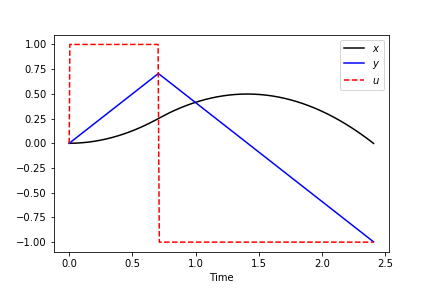
\includegraphics[width=0.5\textwidth]{Exo2Verif.png}
	\caption{Confirmation des résultats pour la 2ème version par comparaison avec la première: $\epsilon=0$, $\xi = 1$, et donc coût$=2.409$}
	\label{fig:Exo2Verif}
\end{figure}

\begin{figure}[H]
    \centering
    \begin{subfigure}[b]{0.32\textwidth}
        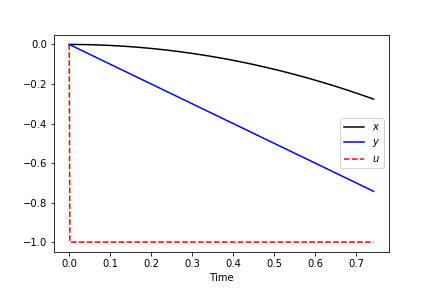
\includegraphics[width=\textwidth]{Exo21.png}
        \caption{$\xi = 0.99$, coût$=0.7362$}
        \label{fig:21}
    \end{subfigure}
    \begin{subfigure}[b]{0.32\textwidth}
        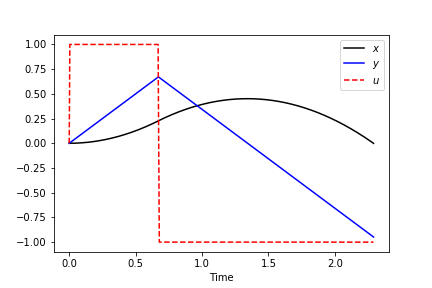
\includegraphics[width=\textwidth]{Exo22.png}
        \caption{$\xi = 0.5$, coût$=1.4714$}
        \label{fig:22}
	\end{subfigure}
    \begin{subfigure}[b]{0.32\textwidth}
        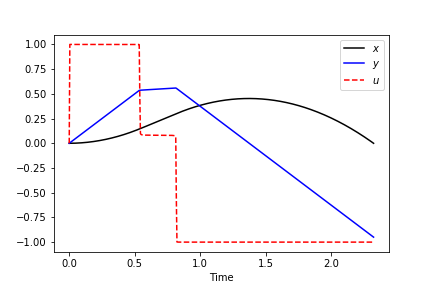
\includegraphics[width=\textwidth]{Exo23.png}
        \caption{$\xi = 0.01$, coût$=0.6669$}
        \label{fig:23}
    \end{subfigure}
       \caption{Résultats obtenus pour $\epsilon= 0.05$}
       \label{fig:epsFaible}
\end{figure}


\begin{figure}[H]
    \centering
    \begin{subfigure}[b]{0.32\textwidth}
        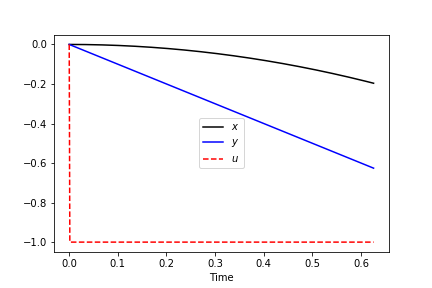
\includegraphics[width=\textwidth]{Exo24.png}
        \caption{$\xi = 0.99$, coût$=0.6199$}
        \label{fig:24}
    \end{subfigure}
    \begin{subfigure}[b]{0.32\textwidth}
        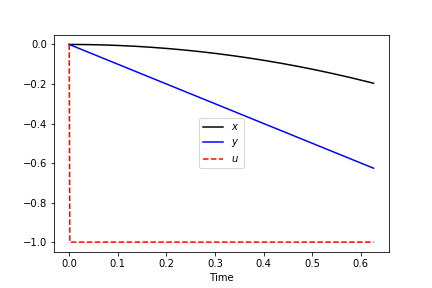
\includegraphics[width=\textwidth]{Exo25.png}
        \caption{$\xi = 0.5$, coût$=0.3298$}
        \label{fig:25}
	\end{subfigure}
    \begin{subfigure}[b]{0.32\textwidth}
        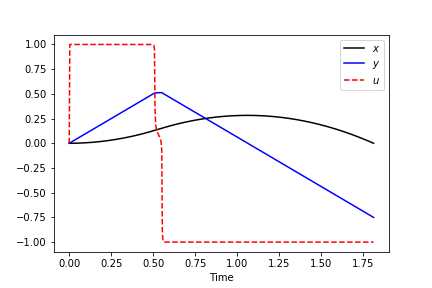
\includegraphics[width=\textwidth]{Exo26.png}
        \caption{$\xi = 0.01$, coût$=0.2700$}
        \label{fig:26}
    \end{subfigure}
       \caption{Résultats obtenus pour $\epsilon= 0.25$}
       \label{fig:epsFort}
\end{figure}

Les \cref{fig:epsFaible,fig:epsFort} permettent de remarquer que la même stratégie qu'à la version 1 est appliquée, vu que le même point d'arrivée est autorisé $\epsilon = 0.05$ ou $= 0.25$. On constate néanmoins une préférence pour la borne supérieure $y(T)=-1+\epsilon$ de l'ensemble d'arrivée, qui est la plus proche de l'état initial $y(0)=0$. 

Aussi, les résultats sont particulièrement dépendants du paramètre $\xi$. En effet, le fait de minimiser une combinaison convexe normalisée du temps final $T$ et de $z(T)$ contraint le système a fondamentalement changer sa stratégie de contrôle (\cref{sub@fig:21,sub@fig:22,sub@fig:23}, ou \cref{sub@fig:24,sub@fig:25,sub@fig:26}).





\clearpage





\section*{Exercice 3 - Contrôle d'insectes}

\subsection*{Question 1}

\begin{problem}
Le problème est modélisé par:
\begin{align}
	\begin{cases}
		x^\prime(t) = x(t)(1-y(t)) \\
		y^\prime(t) = -y(t)(u(t)-x(t))\\
		x(0)=1, y(0)=4
	\end{cases}
	\label{eq:exo3}
\end{align}

Démontrons que, pour tout contrôle $u$, $x(t)>0$ et $y(t)>0$ sur $[0,T]$
\end{problem}

\subsection*{Réponse}
En posant $X(t)=\myvec{x(t)}{y(t)}$, on peut écrire 
\begin{align*}
	\begin{cases}
		X(t)=f(X(t),u(t)) \\
		X(0)=(1,4)
	\end{cases}
\end{align*}

\begin{itemize}
	\item l'application $(X,u)\mapsto f(X(t),u(t))$ mesurable p.p. $t\in [0,T]$ et est continue
	\item $f$ est intégrable en $t$, ou plus précisément en $u(t)$
	\item $f$ est globalement lipschitzienne en $X$
\end{itemize}
Nous sommes donc dans les conditions d'application du théorème de Cauchy-Lipschitz.

\begin{itemize}
	\item[$\blacksquare$] Montrons que $x(\cdot)>0$ p.p.
	Supposons par l'absurde qu'il existe $t_0 \in \mathbb{R}$ tel que $x(t_0)=0$. Alors, $x(t)$ résout le système de Cauchy:
	\begin{align*}
		\begin{cases}
			x^\prime(t) = x(t)(1-y(t)) \\
			y^\prime(t) = -y(t)(u(t)-x(t))\\
			x(t_0)=0,\, y(t_0)=\tilde{y}_0 \in \mathbb{R}
		\end{cases}
	\end{align*}
	Or le couple défini par $\bar{x}(t)\equiv0$ et $\bar{y}^\prime(t)=-y(t)u(t), \hquad \bar{y}(t_0)=\tilde{y}_0$ est solution particulière (globale et maximale) de ce système. Par unicité de la solution d'après le théorème de Cauchy-Lipschitz, on en déduit que $x\equiv\bar{x}\equiv 0$ et $y \equiv \bar{y}$. Ce qui est absurde car la condition initiale du système \eqref{eq:exo3} assure $x(0)=1>0$.
	\item[$\blacksquare$] On procède de manière similaire pour montrer que $y(\cdot)>0$.  
\end{itemize} 

\subsection*{Question 2}
\begin{problem}
	Points d'équilibres du système
\end{problem}
	
\subsection*{Réponse}
On a 
\begin{align*}
	f(X,u)=0 \Rightarrow 
	\begin{cases}
	x(1-y)=0 \\
	y(u-x)=0	
	\end{cases}
	\Rightarrow 
	\begin{cases}
	x=0 \text{ ou } 1-y=0 \\
	\text{et} \\
	y=0 \text{ ou } u-x=0
	\end{cases}
\end{align*}

L'ensemble des points d'équilibre est donc donné, pour $\lambda \in [1;3]$, par l'ensemble des couples $(X_e,u_e)$ tel que 
\begin{align*}
u_e &= \lambda \\
X_e &= \myvec{x_e}{y_e}= \myvec{\lambda}{1}
\end{align*}
La représentation de ces points dans le quadrant $x>0, \, y>0$ est donnée ci-bas:
\begin{figure}[h]
    \centering
    % 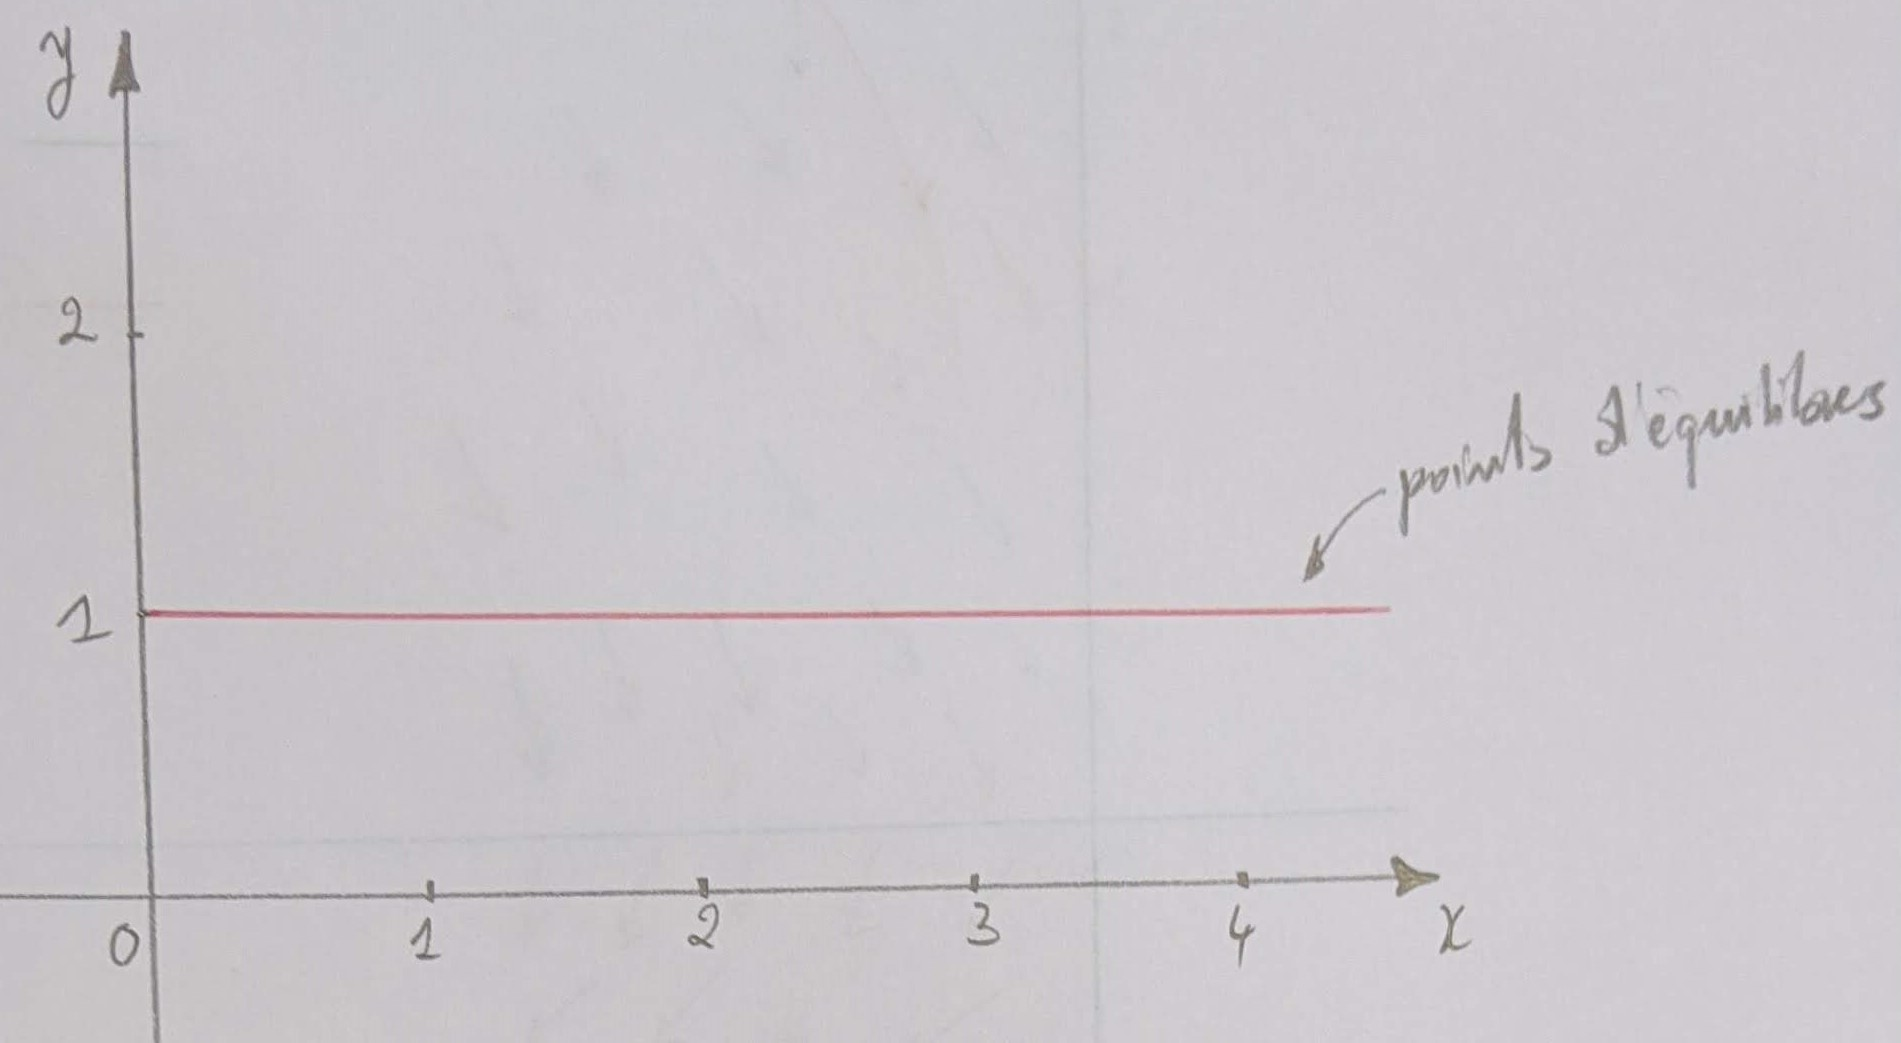
\includegraphics[width=0.7\textwidth]{equilibre.jpg}
    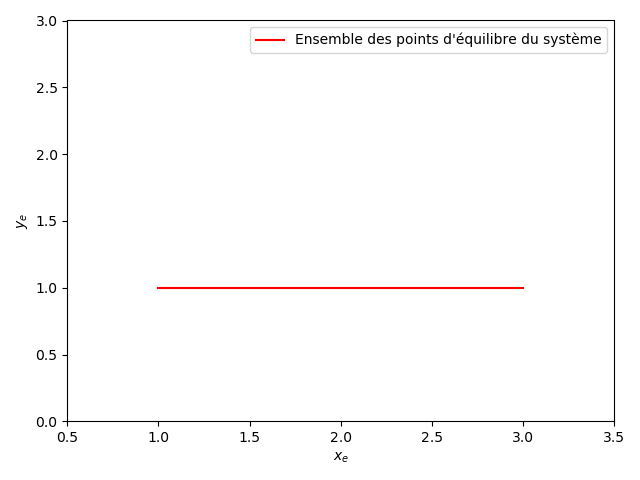
\includegraphics[width=0.5\textwidth]{NewEq.png}
    \caption{Représentation des points d'équilibre du système}
\end{figure}



\subsection*{Question 3}
\begin{problem}
	Portrait de phase de ce système
\end{problem}
	
La méthode employée est la suivante:

\begin{itemize}
	\item On trace l'isocline horizontale
	$$
	\{(x,y) \in \mathbb{R}^2 : x(1-y) = 0 \}
	$$
	On trace ensuite des flèches vers la droite lorsque $x(1-y) > 0$, et vers la droite lorsque $x(1-y) < 0$ 
	\item On trace l'isocline verticale
	$$
	\{(x,y) \in \mathbb{R}^2 : -y(u-x) = 0\}
	$$
	On trace ensuite des flèches vers le haut lorsque $-y(u-x)>0$, et vers le bas lorsque $-y(u-x) < 0$ 
	\item On a donc délimité plusieurs régions du plan. Le "somme" des vecteurs placés dans ces régions nous donne le champ de vecteurs.
	\item La trajectoire est obtenue en localisation la région dans laquelle se trouve $(x_0,y_0)=(1,4)$ et en suivant le champ de vecteur.
\end{itemize}


% \begin{figure}[H]
%     \centering
%     \begin{subfigure}[b]{0.35\textwidth}
%         % \centering
%         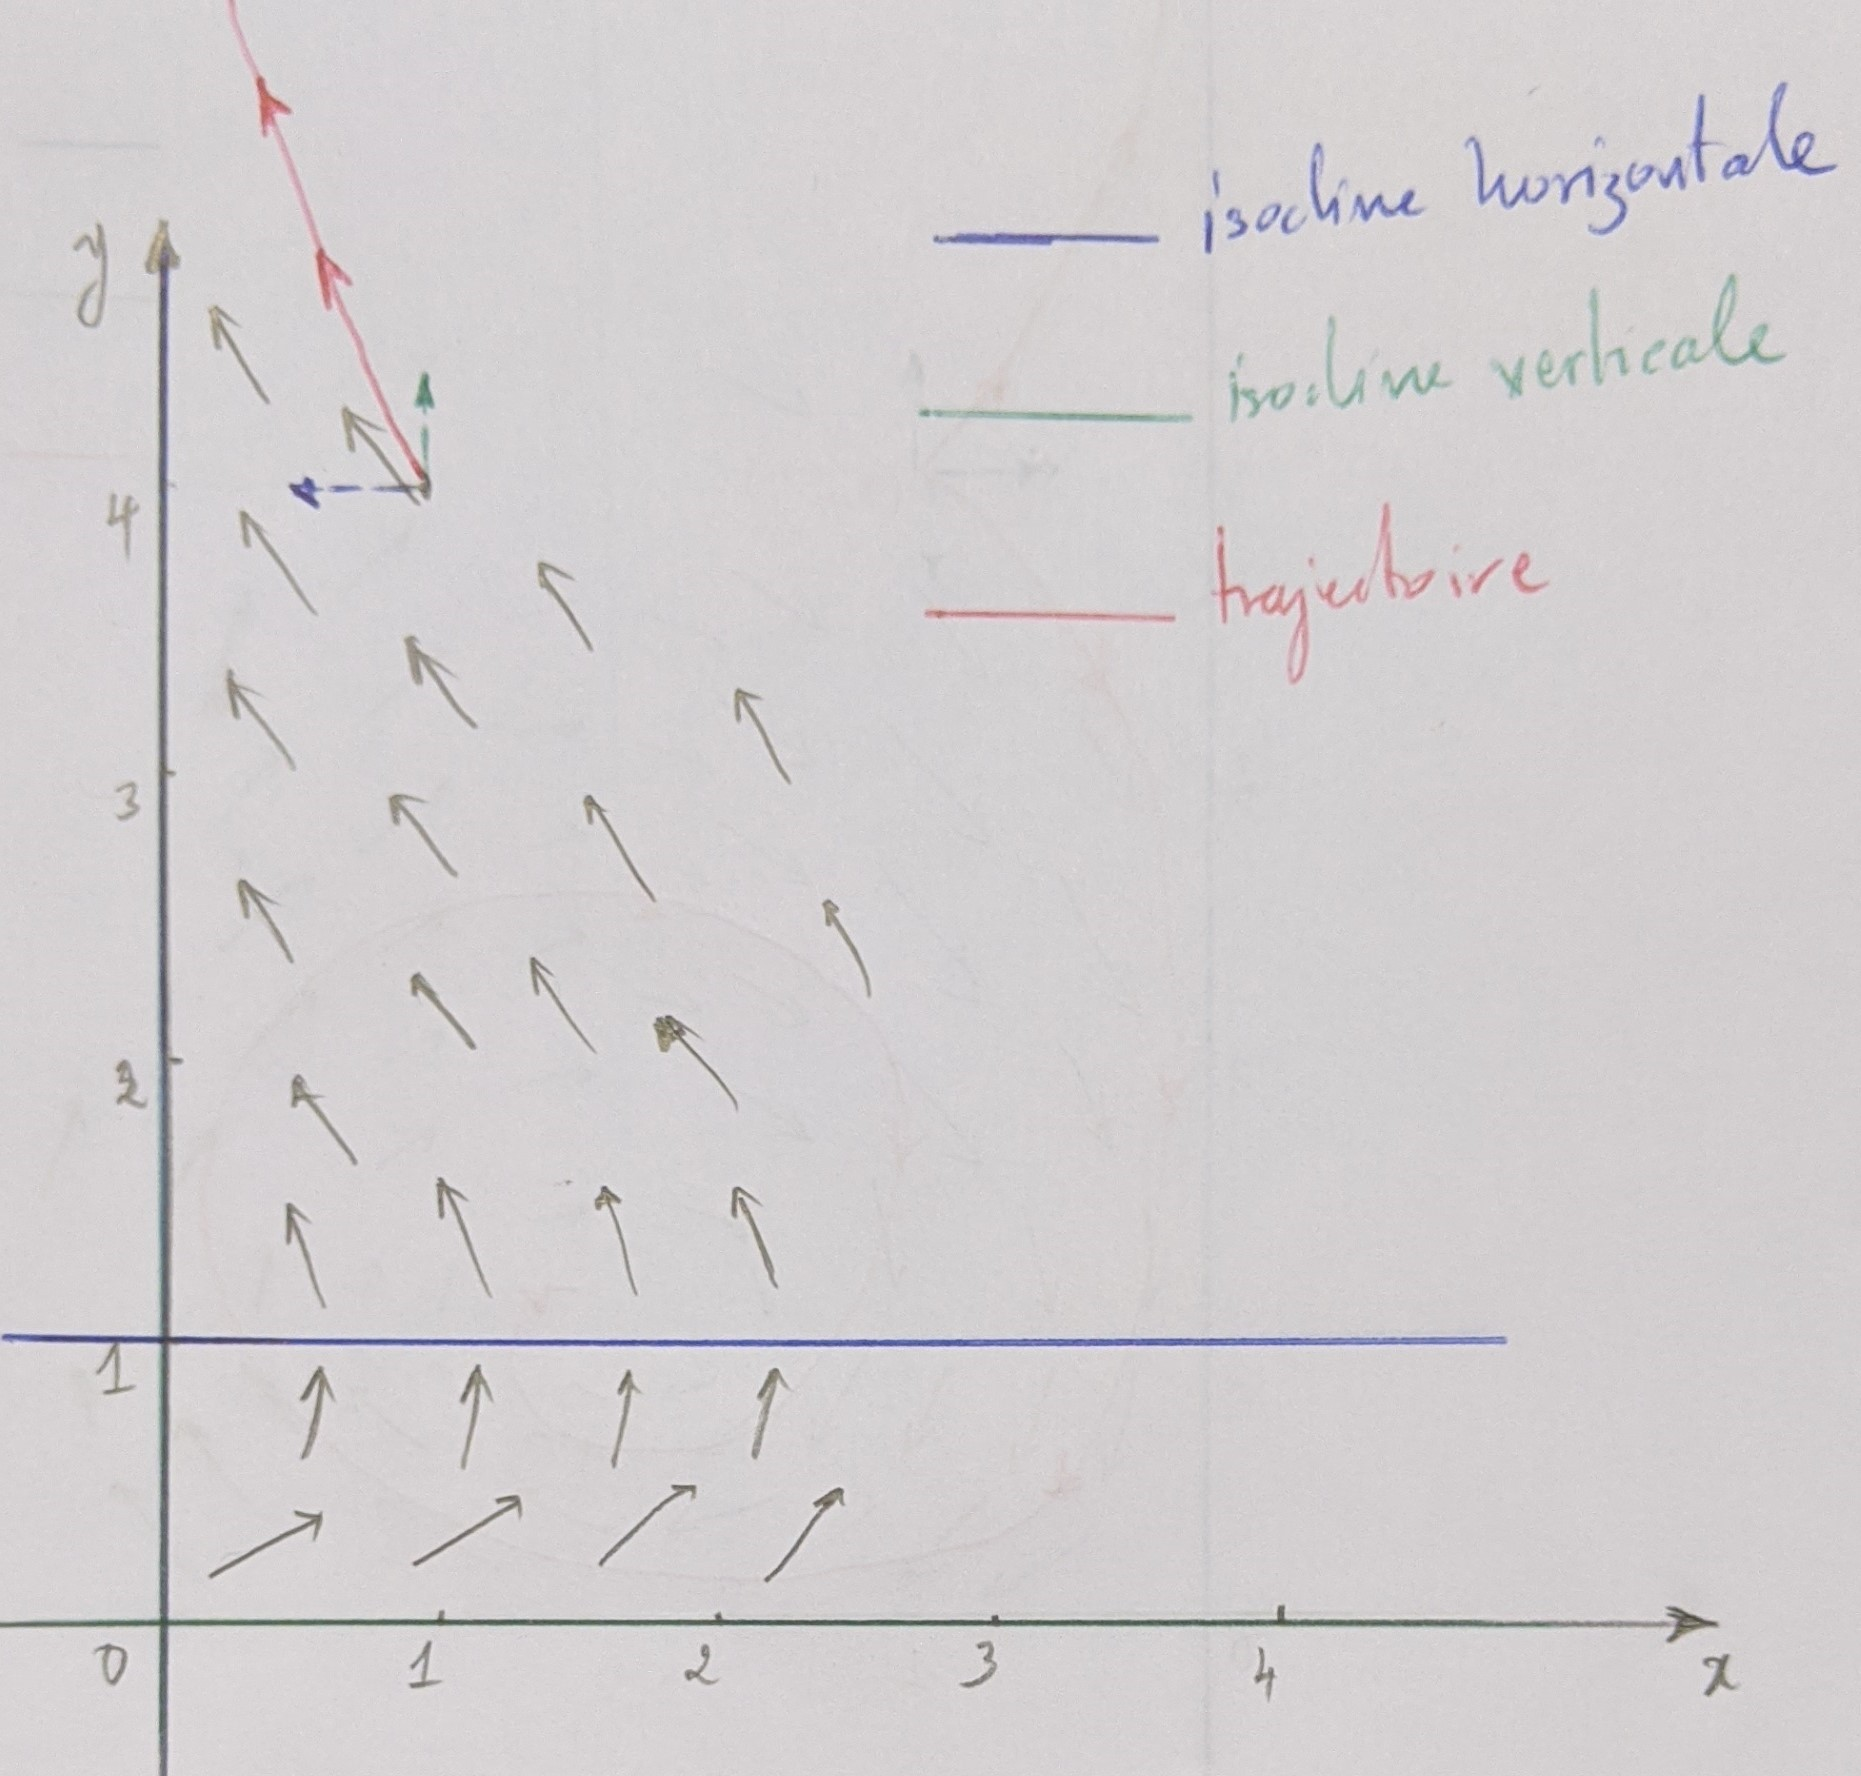
\includegraphics[width=\textwidth]{u0.jpg}
%         \caption{$u(\cdot)=0$}
%         \label{fig:u0}
%     \end{subfigure}
%     % \hfill
%     \begin{subfigure}[b]{0.35\textwidth}
%         % \centering
%         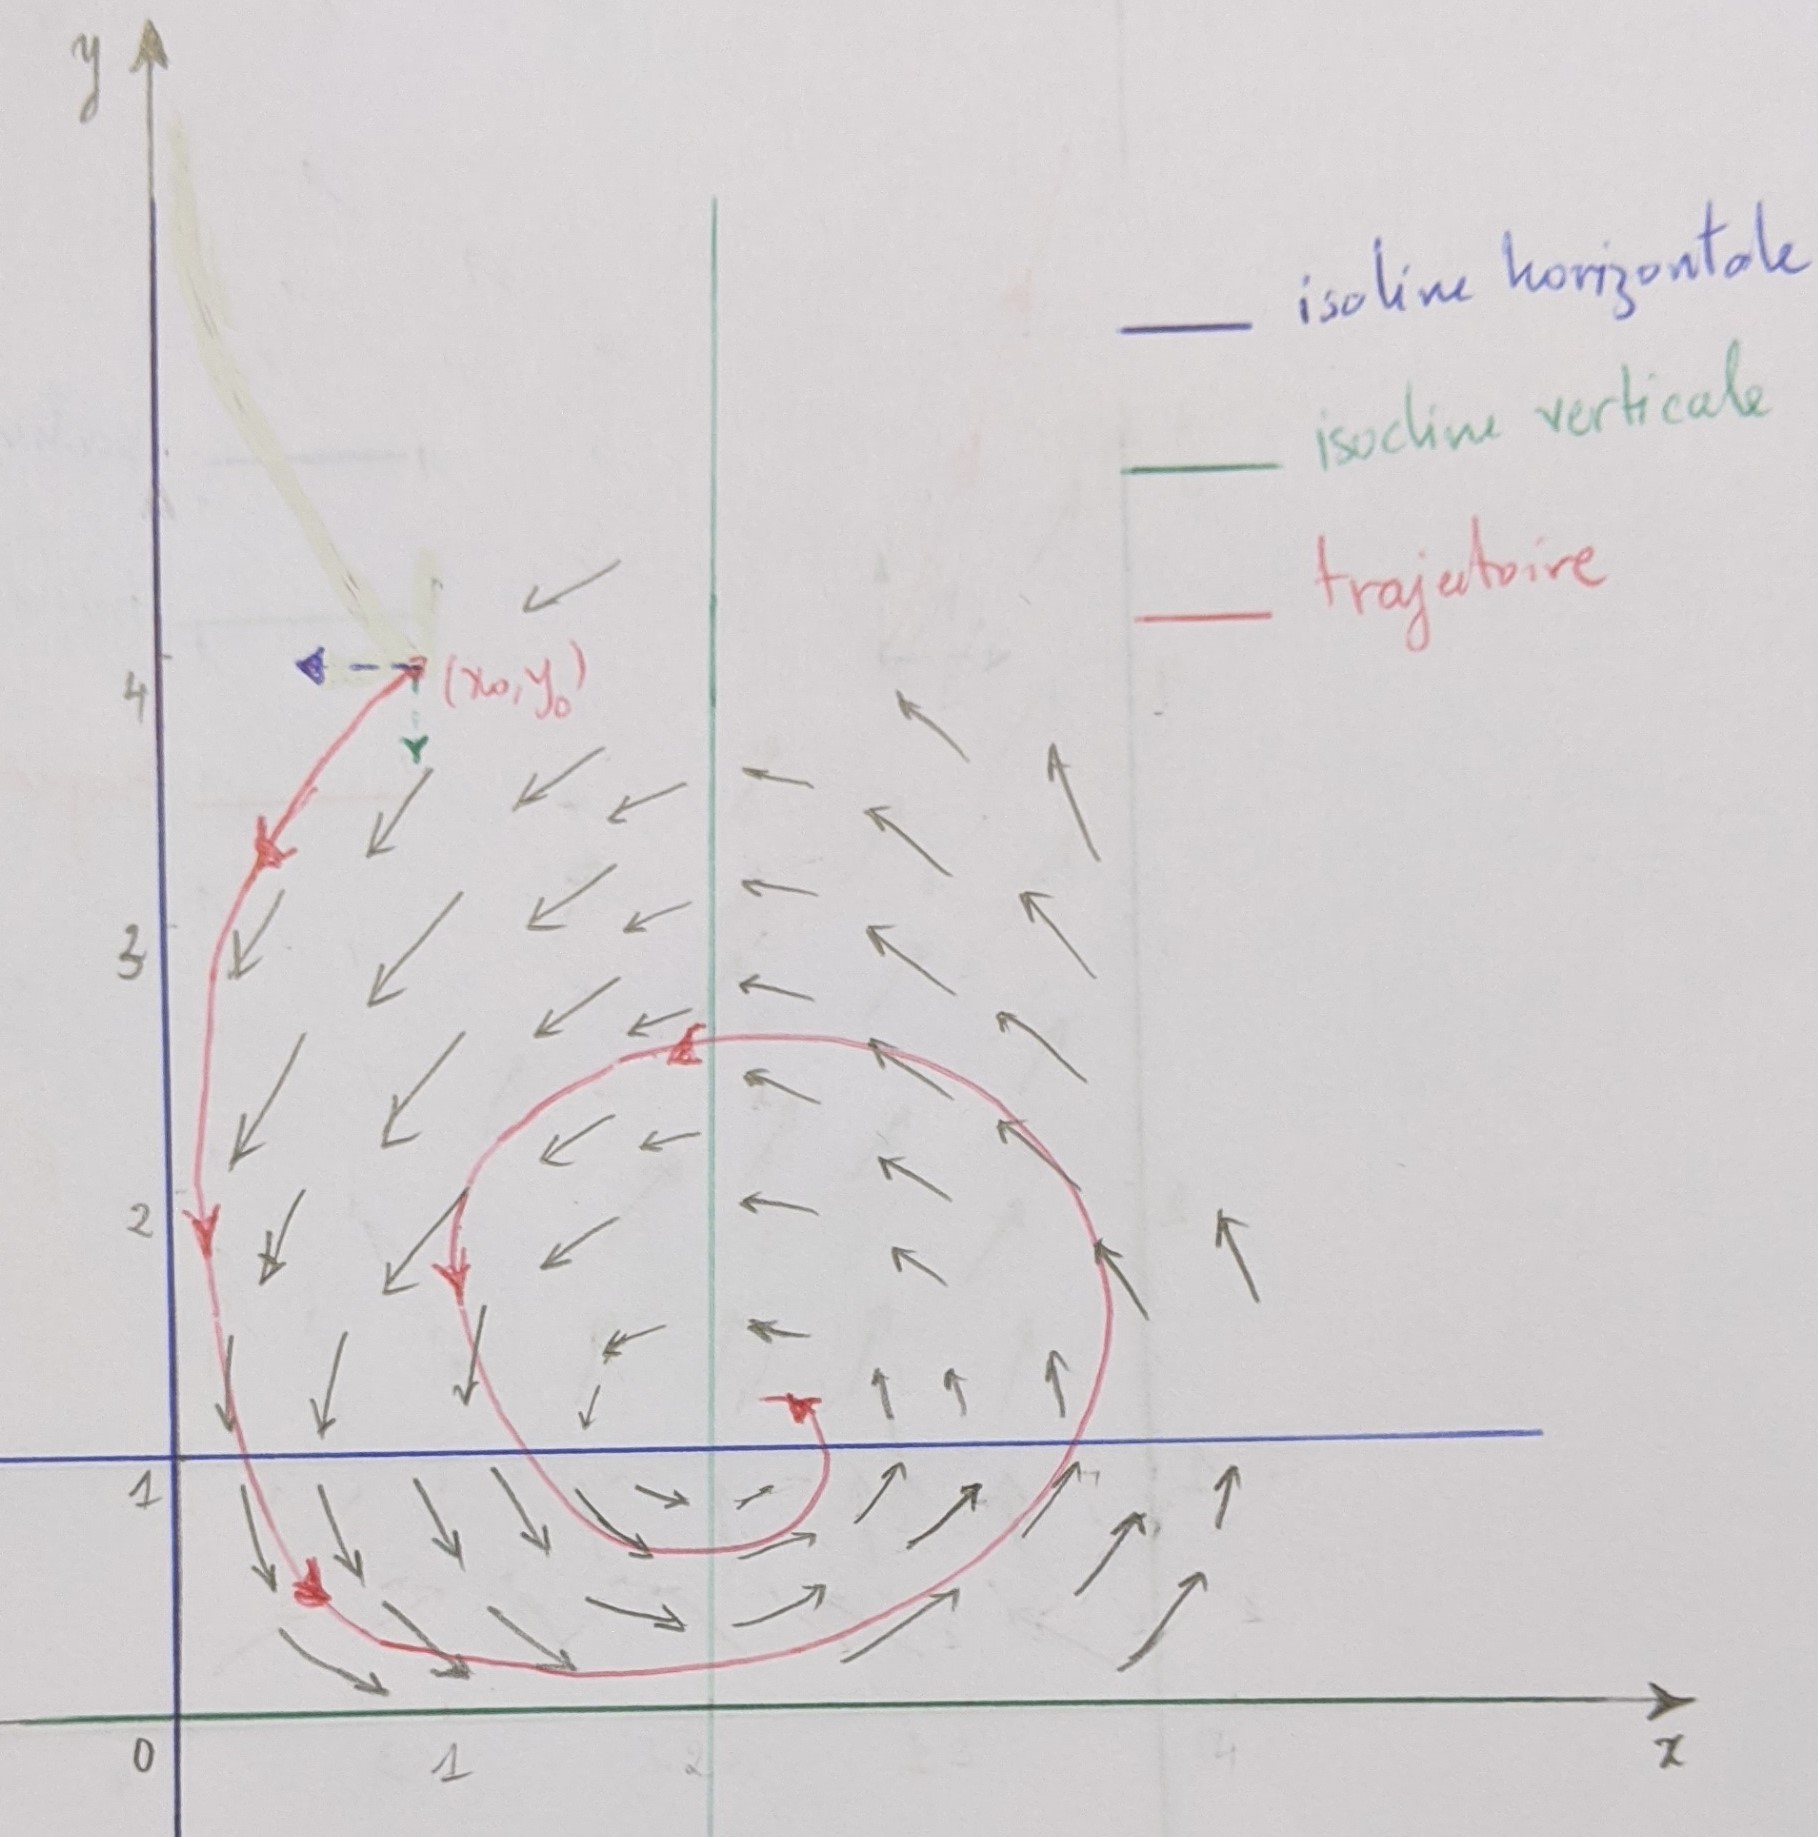
\includegraphics[width=\textwidth]{u2.jpg}
%         \caption{$u(\cdot)=2$}
%         \label{fig:u2}
%     \end{subfigure}
%     % \hfill
%        \caption{Portrait de phases du système. EN abcisse nous avons la population d'insectes nuisibles, et en ordonnées, celle des prédateurs}
%        \label{fig:phase}
% \end{figure}


\begin{figure}[H]
    \centering
	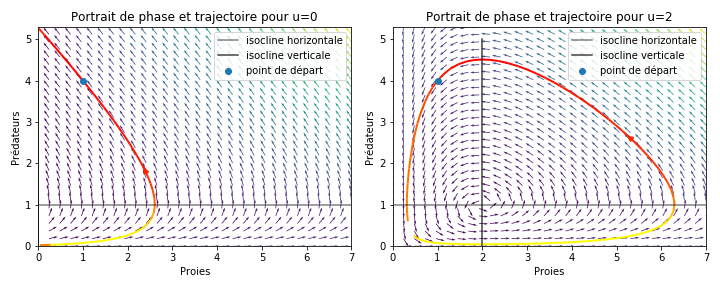
\includegraphics[width=0.8\textwidth]{PhasePy.png}
	\caption{Champs de vecteurs et trajectoires obtenus en utilisant les modules 'quiver' et 'streamplot' de Matplotlib, ceci en interprétant les dérivées $x^\prime(t)$ et $y^\prime(t)$ comme des vitesses. La couleur de la trajectoire (rouge-jaune) indique la quantité de prédateurs dans l'écosystème, sur laquelle on agit directement. À gauche $u\equiv0$, et à droite $u\equiv2$.}
	\label{fig:phase}
\end{figure}

La \cref{fig:phase} permet de remarquer que pour une initialisation au point $(x(0),y(0)) = (1,4)$, le contrôle constant $u\equiv0$ conduit à un état bien précis $(x(T),y(T)) = (0,5.276)$, tandis que le contrôle $u\equiv2$ ne conduit jamais à une convergence. En effet, avec un contrôle constant, le système n'est pas "exactement" contrôlable (les points atteignables étant limitées aux trajectoires indiquée sur les figures). Ce résultat indique que si les prédateurs (qui consomment les insectes nuisibles) périssent eux même à un rythme bien précis $u\equiv2$, alors l'écosystème survivra indéfiniment dans un état dynamique. Par contre si les prédateurs ne disparaissent pas ($u\equiv0$), alors le milieu devient très rapidement inondé de prédateurs, et l'expérience de contrôle d'insectes nuisibles est terminée.


\subsection*{Question 4.1. Résolution numérique (1ère version)}

D'entrée, testons le cas du contrôle constant présenté à la question 3.
\begin{figure}[H]
    \centering
    \begin{subfigure}[b]{0.4\textwidth}
        % \centering
        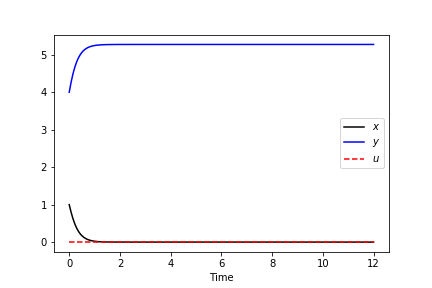
\includegraphics[width=\textwidth]{Exo3Test1.png}
        \caption{$u(\cdot)=0$}
    \end{subfigure}
    % \hfill
    \begin{subfigure}[b]{0.4\textwidth}
        % \centering
        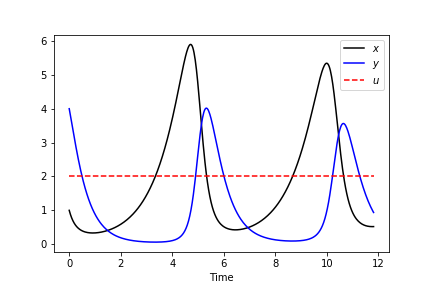
\includegraphics[width=\textwidth]{Exo3Test2.png}
        \caption{$u(\cdot)=2$}
    \end{subfigure}
    % \hfill
       \caption{Trajectoire obtenue par résolution numérique du système avec un contrôle constant}
       \label{fig:Exo3Test}
\end{figure}

La \cref{fig:Exo3Test} permet bien de constater que, pour une initialisation au point $(x(0),y(0)) = (1,4)$, et une destination au point d'équilibre $(x(T),y(T)) = (u,1)$, le contrôle constant $u\equiv0$ n'aboutit pas, mais conduit inévitablement vers $(x(T),y(T)) = (0,5.276)$; il en est de même pour le contrôle $u\equiv2$, sauf qu'il ne conduit à aucun état stable, ceci même après le temps minimal imposé $lower \, bound (T) = 10$. Cette convergence (a) et cette périodicité (b) confirment bien les résultats observés à la \cref{fig:phase}.
 
\begin{figure}[H]
    \centering
    \begin{subfigure}[b]{0.32\textwidth}
        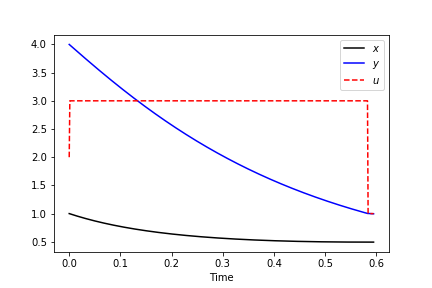
\includegraphics[width=\textwidth]{Exo31.png}
        \caption{$a = 1.05$, $T=0.59447$}
        % \label{fig:21}
    \end{subfigure}
    \begin{subfigure}[b]{0.32\textwidth}
        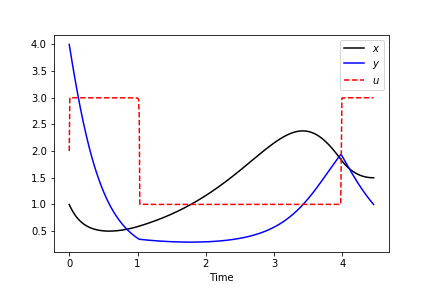
\includegraphics[width=\textwidth]{Exo32.png}
        \caption{$a = 1.5$, $T=4.4553$}
        % \label{fig:21}
	\end{subfigure}
    \begin{subfigure}[b]{0.32\textwidth}
        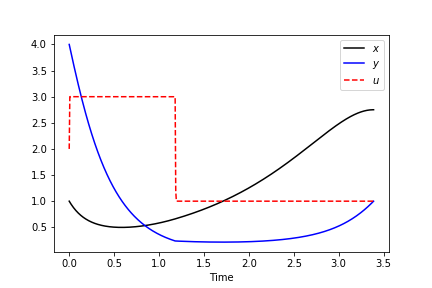
\includegraphics[width=\textwidth]{Exo33.png}
        \caption{$a = 2.75$, $T=3.3886$}
        % \label{fig:21}
    \end{subfigure}
       \caption{Résultats de contrôle d'insecte obtenu pour la première version}
       \label{fig:TempsMin}
\end{figure}

La \cref{fig:TempsMin} montre que l'obtention d'une population d'insectes proche de $1.5$ est la plus difficile. On remarque bien que l'état $x(T)=a=1.05$ est très rapidement atteint, vu qu'il est proche de l'état initial $x(T)=1$. 

\subsection*{Question 4.2. Résolution numérique (2ème version)}

Pour modéliser ce problème, il suffit de poser $z'(t) = u(t)^2$ liée au coût du contrôle d'insectes prédateurs (le coût de la limitation de leur population). On ajoute donc cette contrainte au système \eqref{eq:exo3} pour obtenir
\begin{align*}
	\begin{cases}
		x^\prime(t) = x(t)(1-y(t)) \\
		y^\prime(t) = -y(t)(u(t)-x(t))\\
		z^\prime(t) = u(t)^2 \\
		x(0)=1,\, y(0)=4, \, z(0)=0
	\end{cases}
\end{align*}
Le problème de minimisation est donc $\inf_{u}{T+z(T)}$ tel que $x(T)=a$, $y(T)=1$.

\begin{figure}[H]
    \centering
    \begin{subfigure}[b]{0.32\textwidth}
        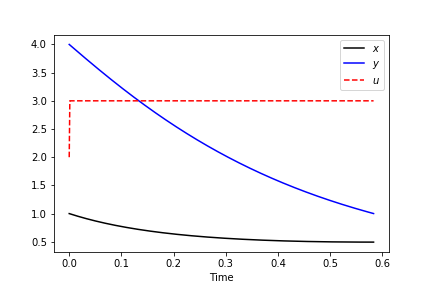
\includegraphics[width=\textwidth]{Exo34.png}
        \caption{$a = 1.05$, coût$=5.8338$}
        % \label{fig:21}
    \end{subfigure}
    \begin{subfigure}[b]{0.32\textwidth}
        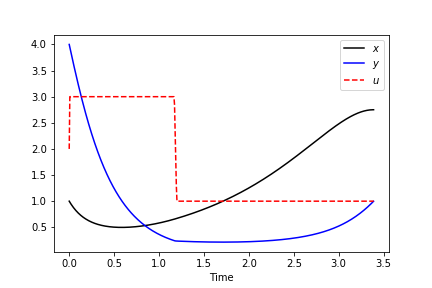
\includegraphics[width=\textwidth]{Exo35.png}
        \caption{$a = 1.55$, coût$=20.1499$}
        % \label{fig:21}
	\end{subfigure}
    \begin{subfigure}[b]{0.32\textwidth}
        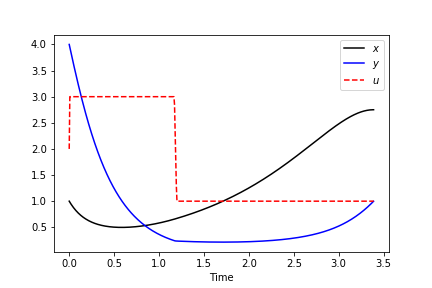
\includegraphics[width=\textwidth]{Exo36.png}
        \caption{$a = 2.75$, coût$=16.197$}
        % \label{fig:21}
    \end{subfigure}
       \caption{Résultats de contrôle d'insecte obtenu pour la deuxième version}
       \label{fig:CoutMin}
\end{figure}

Les résultats de la \cref{fig:CoutMin} permettent de confirmer ceux indiqués plus haut à la \cref{fig:TempsMin}. Dans tous les cas, le contrôle obtenu est bang-bang, indiquant que, ayant introduit un grand nombre de prédateurs initialement ($y(0)=4$), la stratégie la plus efficace (la moins coûteuse) est de \textbf{réduire radicalement la population de prédateurs jusqu'à une valeur critique ($y \approx 0.404$), et puis de ralentir l'extinction, donnant ainsi la chance à ces derniers de se reproduire; une fois qu'il y en a assez, on recommence le processus}. 

% -------------------------------------------------------------------------------
% REFERENCES
% --------------------------------------------------------------------------------
% \section*{References}

\end{document}
